\documentclass[conference]{IEEEtran}
\usepackage{cite}
\usepackage{amsmath,amssymb,amsfonts}
\usepackage{graphicx}
\usepackage{listings}
\usepackage{physics}
\usepackage{caption}
\usepackage{stfloats}

\begin{document}

\title{Factoring RSA keys with Shor's algorithm}

\author{\IEEEauthorblockN{Giulio Muscarello}}

\maketitle

\begin{abstract}
RSA is a well-known public cryptography scheme that relies on the integer factorization problem. Shor's algorithm, first described in 1994, factorizes integers in polynomial time using a quantum computer. We present an improvement to the Qiskit implementation of Shor's algorithm and demonstrate an attack on communications protected by RSA.
\end{abstract}

\section{Introduction}
We know from the fundamental theorem of arithmetic that every positive integer has a unique prime factorization. There are no known classical algorithms that can factor integers in polynomial time; in fact, the problem of whether such an algorithm exists is known as the "integer factorization problem". Many cryptographic schemes are based on the difficulty of factoring composite integers. Among them, RSA is the most common cryptosystem.

Shor proved \cite{shor} that quantum computers can solve the factorization problem in linear time, and developed an algorithm for this purpose. The impact of quantum computers on the security of encrypted data and communications is therefore a key concern in the security community, and the development of so-called "post-quantum cryptography" is an active area of research. This paper presents a demonstration of Shor's algorithm to attack a toy RSA example.

\section{Algorithms}
\subsection{RSA}
RSA is an asymmetric cryptosystem, meaning that it produces a "public key" and a "private key". Any person can thus encrypt a message using the receiver's public key, and the receiver can decrypt it with his private key. Today RSA sees wide implementation, securing all sorts of communications from Internet browsing to e-mail traffic to instant messaging.

A mathematical description of RSA is out of scope for this paper, and can be found in \cite{rsa}. For the purposes of this paper, the cryptosystem can be thought of as a private key $\{p, q\}$, where $p$ and $q$ are primes known only to the receiver, and a public key $N=pq$, which can be disseminated. The public key allows any third party to encrypt messages, and the private key allows the receiver to decrypt messages intended for him.

\subsection{Reduction to the order-finding problem}
Miller \cite{miller} proved that the problem of factoring $N$ can be reduced to the "period-finding problem": for a given $a < N - 1$, find the smallest $r$ such that $a^r \equiv 1 \mod N$ (i.e. find the order of the algebraic group of integers coprime with $N$ and smaller than $N$, hence the name of "order-finding problem" by which it is found in literature). Specifically, depending on the choice of $a$ we have that either:
\begin{itemize}
\item $N$ and $a$ have a common prime factor, in which case $p=\gcd(N, a)$ returns one prime and $N/p$ returns the other;
\item let $r$ be the period defined above, then at least one of $p, q = \gcd(N, a^{r/2}\pm 1)$ are factors of $N$;
\item neither hold, we had a "bad" choice of $a$.
\end{itemize}

It can be shown that in the generic case where $N$ has $k$ prime factors, the algorithm above yields a factor with probability $p=1-2^{1-k}$; in the case of RSA, $p=0.5$.

The random choice of $a$ and the computation of possible factors is known as the "classical part" of Shor's algorithm. The solution to the period-finding problem however is of greater theoretical interest, and can be solved by the quantum algorithm that is at the core of Shor's algorithm.

\subsection{Order-finding subroutine}\label{order-finding}
The key insight in Shor's algorithm is that the order-finding problem can be expressed in terms of finding the eigenvalues of a unitary operator, a problem which can be solved with the quantum phase estimation algorithm in $O((\log N)^3)$, i.e. linearly in the number of bits of $N$. For comparison, the best classical algorithm for factoring has a complexity of $O(e^{(\log N)^{1/3}(\log\log N)^{2/3}})$.

Shor exploits the unitary operator
\begin{equation}
U_a: x \rightarrow ax \mod N
\end{equation}
whose eigenvalues\footnote{The reader can prove this by substitution: the eigenvectors take the form $\frac{1}{\sqrt{r}}\sum_{m=0}^{r-1}\exp(\frac{-2\pi i m n}{r})\ket{x^k \mod N}$.} are a function of $r$:
\begin{equation}
e^{2i\pi k/r}\text{ for some integer }k
\end{equation}

The phase estimation algorithm can estimate $\theta=k/r$ to within a given error $\epsilon$: it returns $\widetilde\theta \in (\theta-\epsilon, \theta+\epsilon)$. We then need to minimize the error to a point where classical algorithms (in this case, continued fraction expansion) can recover $\theta$ from $\widetilde\theta$.

Because the candidates for $k/r$ are so close to one another (in the worst case, $1/N$ apart) and the number of gates is $O(1/\epsilon)$, direct application of the phase estimation algorithm is cost-prohibitive. We instead use a mathematical trick to increase accuracy at no additional cost.

Consider the family of unitary operators
\begin{equation}
U_a, U_{(a^2)}, U_{(a^4)}, U_{(a^8)}...
\end{equation}
All such operators $U_b$ are integer powers of $U_a$: it is easy to verify that if $b = a^n$ then $U_b = (U_a)^n$. For this reason they have the same eigenvectors, but despite being integer powers they are only as hard to implement as $U_a$, since one need only precompute $a^n \mod N$ by repeated squaring. Their eigenvalues, however, have far lower error than $U_a$: note that if $U_a$ has an eigenvalue $e^{i\phi}$, then $U_{(a^2)}$ has an eigenvalue $e^{2i\phi}$, $U_{(a^4)}$ has an eigenvalue $e^{4i\phi}$, and so on. The QPE will then estimate $\phi$, $2\phi$, $4\phi$... to within the same error $\epsilon$, thus reducing the error on $\phi$ to $\epsilon$, $\epsilon/2$, $\epsilon/4$...

It can be shown that for the purposes of determining $r$ it is sufficient to estimate a few randomly picked eigenvalues with a precision smaller than $1/N^2$, which corresponds to measuring the eigenvalues for all $U_b$ until $b=a^{(2^p)}$, $2^p \approx N^2$.

\subsection{Modular exponentiation}
The modular exponentiation procedure is at the heart of Shor's algorithm, and can be implemented in several ways. Notably, any classical computation (thus including modular exponentiation) can be expressed in terms of Toffoli gates, as they are universal for Boolean functions --- for an example of such a general approach, see \cite{toffoli}. However, in literature we can find specialized circuits for modular exponentiation, the first being described in a paper \cite{vbe} by Vedral, Barenco and Ekert and still used today in Qiskit's implementation of Shor's algorithm.

\section{Demonstration}
We now demonstrate the use of Shor's algorithm to decrypt a RSA key and thus read the contents of a communication encrypted with RSA. Specifically, we will use the implementation contained in Qiskit, a mainstream open-source framework for quantum computing.

\subsection{RSA}
RSA keys are typically 1024 or 2048 bits long, with some being 3072 or 4096 bits long. However, factoring such large keys with Shor's algorithm is computationally infeasible, and practical concerns require us to use extremely small keys (around $N=30$ at most). The resulting circuits are otherwise too large and can take several minutes or hours to compute: empirically, we observe that a circuit for $N=33$ is executed in 10 minutes on the powerful IBM QASM simulator. Needless to say, such small keys provide no actual security as they can be factored by hand, and only serve as a demonstration in place of larger keys.

Mainstream RSA implementations are designed with reasonable minimum key sizes: for instance, OpenSSL requires 384 bits or more, and will fail with an error for shorter keys. This requirement partly stems from the use of padding schemes, which add desirable security properties such as non-determinism (the same message encrypted several times will have several different encryptions; this is not true with plain RSA), preventing partial decryption, and others. As we only want to explore the feasibility of factoring the RSA key, such security properties are not of interest to us, and we can use a custom RSA implementation with tiny keys and no padding scheme.

\subsection{Shor}
We use the implementation of Shor's algorithm from the Qiskit library. The implementation uses the techniques outlined in section \ref{order-finding}, where the modular exponentiation circuit used to construct $U_b$ is derived in \cite{vbe}.

We present a dramatic improvement upon this algorithm that brings the time spent constructing the circuit from 127 seconds (using Qiskit's implementation at the time of writing) to 6 seconds for $N=33$. The resulting circuit is identical and thus has the same execution time; this improvement merely makes the circuit construction faster.

Simple line profiling shows that the Qiskit implementation spends a large amount of time composing subcircuits together (for instance, appending an IQFT circuit as part of the QPE routine). Delving into the library code shows that the composition of circuits is implemented by transforming the operands into DAGs\footnote{DAG: Directed Acyclic Graph.}, merging those, and then retransforming back into a circuit. We report an abridged version of the method:

\lstset{basicstyle=\ttfamily\footnotesize,breaklines=true}
\begin{lstlisting}[language=Python]
def compose(self, other):
        dag_self = circuit_to_dag(self)
        dag_other = circuit_to_dag(other)
        dag_self.compose(dag_other)
        return dag_to_circuit(dag_self)
\end{lstlisting}

Further profiling shows that the conversion from and to DAGs is very computationally intensive with respect to the other steps. The key intuition is that sequential compositions are therefore wasteful, as they spend a lot of time converting intermediate values back and forth; representing them as DAGs instead, only converting to and from DAGs respectively at the beginning and at the end of the algorithm, allows for much more efficient composition. In reality the composition takes additional arguments (most importantly the qubit indices on which to compose), which need to be stored along with the DAG - we call this object a "tagged DAG". This simple modification then allows to construct the circuit correctly with dramatic speed improvements.

This improvement was discovered independently by Thomas Metcalfe, who submitted it in a slightly different form on May 25 as part of pull request \#975 to Qiskit Aqua. As the PR is not yet merged at the time of writing, we have released our implementation \cite{github-repo-shor} as a separate repository.

\subsection{Application}
We develop a simple client-server application that emulates an email service. Users can log in with their username and password, and once logged in they can browse their email messages. It uses a simple cryptographic protocol that simulates TLS, where the server sends its public key to the client, which in turn sends an encrypted AES key (a "session key") allowing for secure two-way communication. The goal of this demonstration is to capture the public key and factor it, allowing a third party to decrypt messages intended for the server and snoop on the credentials and the email messages.

We have released the code for the demonstration, together with this paper, as a public Git repository \cite{github-repo-main}.

\section{Results and conclusions}
We demonstrate that Shor's algorithm can be used to factor RSA keys and compromise encrypted channels. We present three cases:
\begin{itemize}
\item $N=15$, factored on a local simulator (Aer backend) in a few seconds;
\item $N=21$, factored on the IBM QASM simulator in 40 seconds;
\item $N=33$, which gave inconclusive results after approximately 10 minutes on the IBM QASM simulator.
\end{itemize}

We notice that with the increase of $N$ the circuit depth and the execution times rise greatly, making local simulation impractical after a certain point. However, even powerful simulators like the one provided by IBM struggle to factor even modest values of $N$, which in turn are extremely tiny in comparison to keys used in the real world (the smaller ones being 1024 bit long).

While performance issues could in theory be addressed with real quantum computers with sufficiently many qubits, we also observe that the demonstration often fails for $N=33$. We attribute this to the large amount of noise and decoherence accumulated in the computation.

Overall, we find that Shor's algorithm is a simple and well-studied method to solve the factoring problem, but at the current time it is vastly unfeasible as a tool against real RSA keys due to the limits of current quantum computing technology.

\begin{figure*}[b]
   \centering
   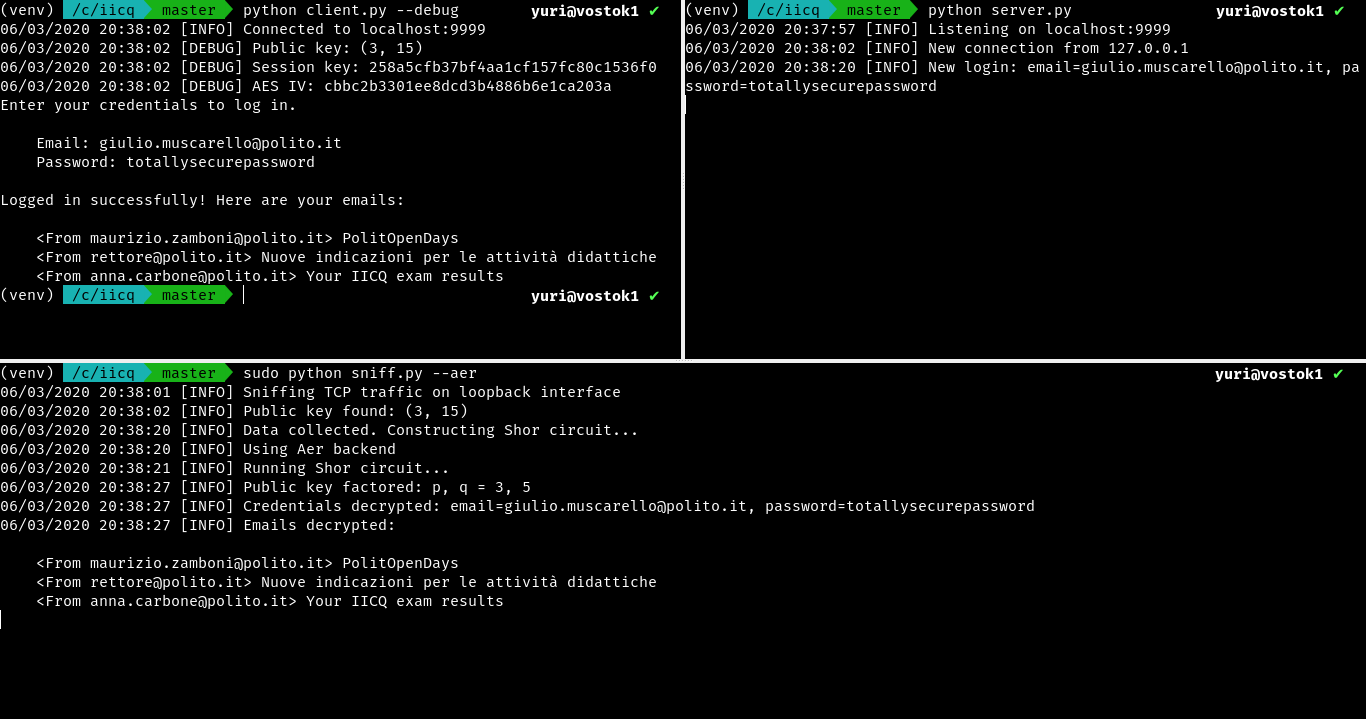
\includegraphics[width=\textwidth,height=\textheight,keepaspectratio]{2020-06-03_20-38.png}
   \caption{A demonstration of the attack on the public key $e=3$, $N=15$. The algorithm was executed on a local simulator (Aer backend); the timestamps show that the factorization was carried out in a few seconds.\\Top left: the client interface. Top right: the server interface. Bottom: the attacker interface.}
\end{figure*}

\begin{figure*}[t]
   \centering
   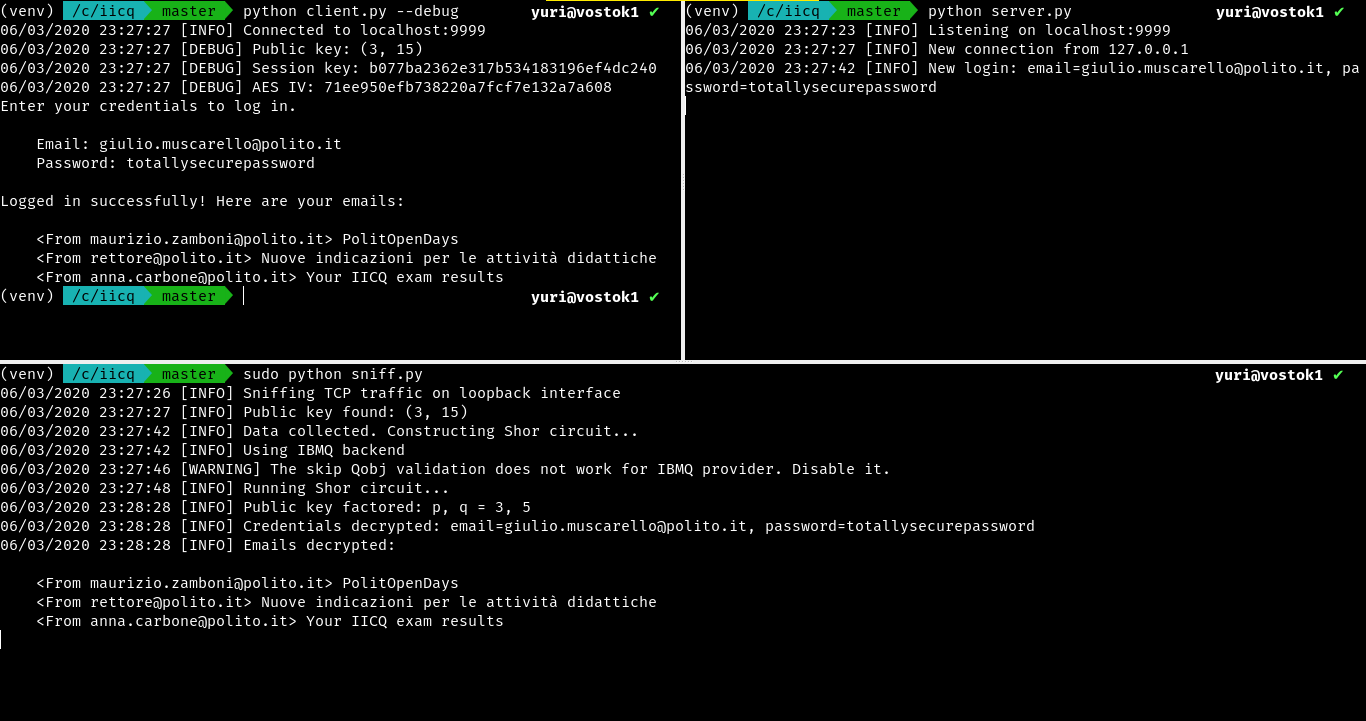
\includegraphics[width=\textwidth,height=\textheight,keepaspectratio]{2020-06-03_23-29.png}
   \caption{A demonstration of the attack on the public key $e=3$, $N=21$. The algorithm was executed on the IBM QASM simulator.}
\end{figure*}

\begin{figure*}[t]
   \centering
   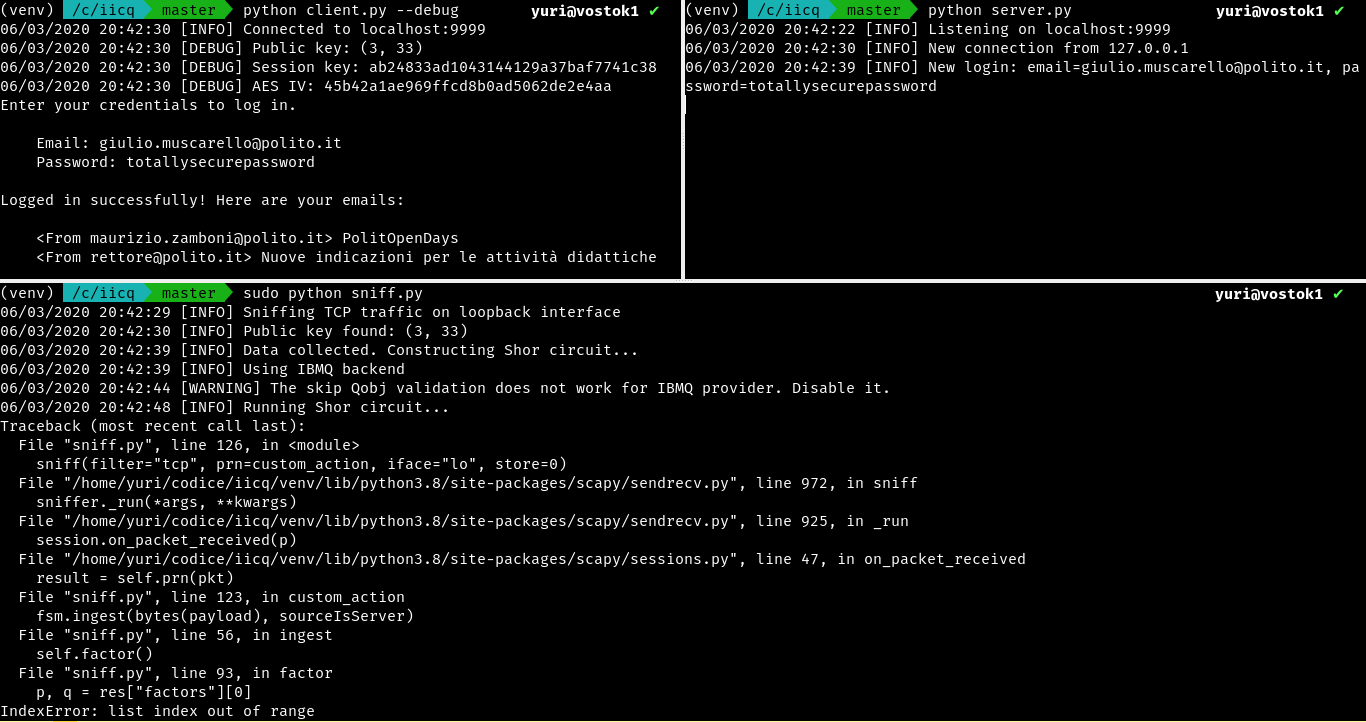
\includegraphics[width=\textwidth,height=\textheight,keepaspectratio]{2020-06-03_20-54.png}
   \caption{A demonstration of the attack on the public key $e=3$, $N=33$. The algorithm was executed on the IBM QASM simulator, and gave inconclusive results.}
\end{figure*}

\begin{figure*}[t]
   \centering
   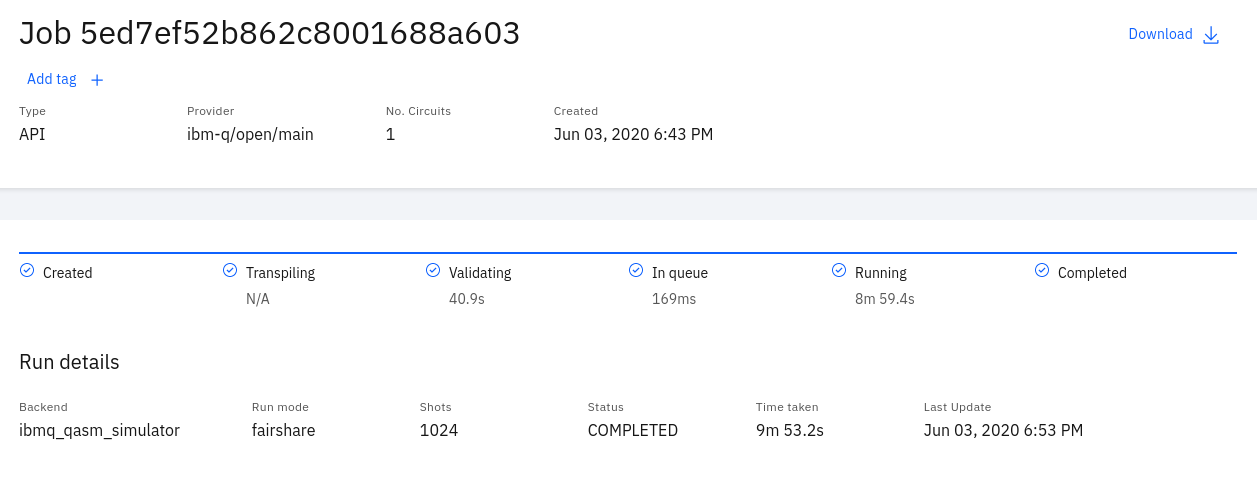
\includegraphics[width=\textwidth,height=\textheight,keepaspectratio]{2020-06-03_20-56.png}
   \caption{Timings for factorizing $pq=33$ on the IBM QASM simulator.}
\end{figure*}

\begin{thebibliography}{00}
\bibitem{shor} P. W. Shor, "Algorithms for quantum computation: discrete logarithms and factoring", SIAM J.Sci.Statist.Comput. 26
\bibitem{rsa} R. Rivest, A. Shamir, L. Adleman, "A Method for Obtaining Digital Signatures and Public-Key Cryptosystems", Communications of the ACM 21
\bibitem{miller} G. L. Miller, "Riemann's hypothesis and tests for primality", J. Comput. System Sci.
\bibitem{vbe} V. Vedral, A. Barenco, A. Ekert, "Quantum Networks for Elementary Arithmetic Operations", Physical Review A 54
\bibitem{toffoli} D. Maslov, G. W. Dueck, D. M. Miller, "Toffoli network synthesis with templates," IEEE Transactions on Computer-Aided Design of Integrated Circuits and Systems
\bibitem{ibm} IBM, "Shor's algorithm",\\https://quantum-computing.ibm.com/docs/guide/q-algos/shor-s-algorithm
\bibitem{github-repo-main} G. Muscarello, https://github.com/CapacitorSet/shor-demonstration
\bibitem{github-repo-shor} G. Muscarello, https://github.com/CapacitorSet/qiskit-fast-shor
\end{thebibliography}
\vspace{12pt}


\end{document}
